\documentclass[tikz, border=10pt]{standalone}
\usepackage{tikz}
\usetikzlibrary{calc}

\begin{document}
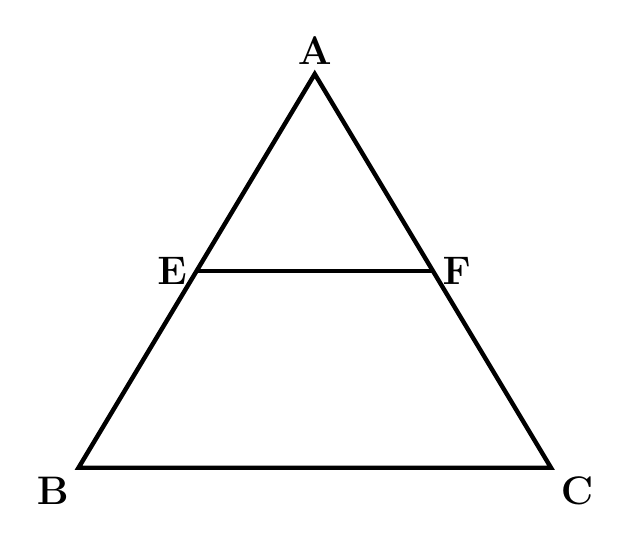
\begin{tikzpicture}

% Define vertices of main triangle
\coordinate (A) at (3, 5);
\coordinate (B) at (0, 0);
\coordinate (C) at (6, 0);

% Define D and E on sides AB and AC (parallel to BC)
\coordinate (E) at ($(B)!0.5!(A)$);
\coordinate (F) at ($(C)!0.5!(A)$);

% Draw the main triangle ABC
\draw[ultra thick] (A) -- (B) -- (C) -- cycle;

% Draw the parallel line DE
\draw[ultra thick] (E) -- (F);

% Labels for vertices
\node[above] at (A) {\textbf{\Large A}};
\node[below left] at (B) {\textbf{\Large B}};
\node[below right] at (C) {\textbf{\Large C}};
\node[right] at (F) {\textbf{\Large F}};
\node[left] at (E) {\textbf{\Large E}};



\end{tikzpicture}
\end{document}